\chapter{Исследовательский раздел}

Был проведен одновременный тест производительности трех экземпляров системы управления базами данных PostgreSQL без ограничений дискового ввода-вывода и с ограничениями. Результатами исследования является количество транзакций в секунду на трех экземплярах для двух тестовых случаев:

\begin{enumerate}
	\item ввод-вывод не ограничен;
	\item ввод-вывод ограничен на всех экземплярах.
\end{enumerate}

Характеристики оборудования, на которых производились замеры следующие.

\begin{itemize}
\item Процессор: Apple M1 Pro~\cite{mac}.
\item Объем оперативной памяти: 16ГБ~\cite{mac}.	
\end{itemize}

Каждый экземпляр PostgreSQL запускался в отдельном контейнере в Kubernetes, для каждого контейнера были выделены следующие ограничения.

\begin{itemize}
\item Процессорное время: 2 единицы~\cite{resource_management}.
\item Объем оперативной памяти: 3ГБ.	
\end{itemize}

Манифест запуска экземпляров PostgreSQL представлен в Приложении~Д.

Манифест с ограничениями дискового ввода-вывода экземпляров представлен в Приложении~Е.

Для теста производительности использовалась утилита \texttt{pgbench}. Для тестирования вызывался \texttt{pgbench} с параметрами, показанными в листинге~\ref{lst:pgbench}.

\begin{lstlisting}[language=Go,label=lst:pgbench, caption={Параметры pgbench}]
pgbench -i -s 100
pgbench  -c 8 -j 2 -T 120
\end{lstlisting}

\section{Результаты}

Было проведено 10 замеров. Результаты измерений без ограничений дискового ввода-вывода представлены в таблице~\ref{tab:res_without}.


\begin{table}[H]
\caption{Результаты измерений без ограничений дискового ввода-вывода}
\label{tab:res_without}
\begin{center}
\begin{tabular}{|l|r|r|r|}
\hline
\multicolumn{1}{|c|}{\textbf{№ замера}} & \multicolumn{1}{c|}{\textbf{\begin{tabular}[c]{@{}c@{}}Экземпляр 1, \\ TPS\end{tabular}}} & \multicolumn{1}{c|}{\textbf{\begin{tabular}[c]{@{}c@{}}Экземпляр 2, \\ TPS\end{tabular}}} & \multicolumn{1}{c|}{\textbf{\begin{tabular}[c]{@{}c@{}}Экземпляр 3, \\ TPS\end{tabular}}} \\ \hline
1                                       & 1590                                                                                      & 1565                                                                                      & 1622                                                                                      \\ \hline
2                                       & 1625                                                                                      & 1619                                                                                      & 1599                                                                                      \\ \hline
3                                       & 1474                                                                                      & 1481                                                                                      & 1509                                                                                      \\ \hline
4                                       & 1645                                                                                      & 1694                                                                                      & 1668                                                                                      \\ \hline
5                                       & 1406                                                                                      & 1432                                                                                      & 1564                                                                                      \\ \hline
6                                       & 1584                                                                                      & 1534                                                                                      & 1503                                                                                      \\ \hline
7                                       & 1563                                                                                      & 1571                                                                                      & 1497                                                                                      \\ \hline
8                                       & 1528                                                                                      & 1493                                                                                      & 1431                                                                                      \\ \hline
9                                       & 1475                                                                                      & 1762                                                                                      & 1731                                                                                      \\ \hline
10                                      & 1683                                                                                      & 1671                                                                                      & 1697                                                                                      \\ \hline
\end{tabular}
\end{center}
\end{table}


\newpage

Результаты измерений c ограничениями дискового ввода-вывода представлены в таблице~\ref{tab:res_with}.

\begin{table}[H]
\caption{Результаты измерений с ограничениями дискового ввода-вывода}
\label{tab:res_with}
\begin{center}
\begin{tabular}{|l|r|r|r|}
\hline
\multicolumn{1}{|c|}{\textbf{№ замера}} & \multicolumn{1}{c|}{\textbf{\begin{tabular}[c]{@{}c@{}}Экземпляр 1, \\ TPS\end{tabular}}} & \multicolumn{1}{c|}{\textbf{\begin{tabular}[c]{@{}c@{}}Экземпляр 2, \\ TPS\end{tabular}}} & \multicolumn{1}{c|}{\textbf{\begin{tabular}[c]{@{}c@{}}Экземпляр 3, \\ TPS\end{tabular}}} \\ \hline
1                                       & 1569                                                                                      & 1542                                                                                      & 1597                                                                                      \\ \hline
2                                       & 1570                                                                                      & 1592                                                                                      & 1566                                                                                      \\ \hline
3                                       & 1539                                                                                      & 1562                                                                                      & 1601                                                                                      \\ \hline
4                                       & 1585                                                                                      & 1602                                                                                      & 1573                                                                                      \\ \hline
5                                       & 1551                                                                                      & 1608                                                                                      & 1531                                                                                      \\ \hline
6                                       & 1568                                                                                      & 1533                                                                                      & 1584                                                                                      \\ \hline
7                                       & 1524                                                                                      & 1581                                                                                      & 1597                                                                                      \\ \hline
8                                       & 1597                                                                                      & 1540                                                                                      & 1539                                                                                      \\ \hline
9                                       & 1580                                                                                      & 1539                                                                                      & 1602                                                                                      \\ \hline
10                                      & 1556                                                                                      & 1571                                                                                      & 1588                                                                                      \\ \hline
\end{tabular}
\end{center}
\end{table}


Результаты измерений представлены в формате гистограммы на рисунке~\ref{img:plot}.

\begin{figure}[h!]
    \centering
    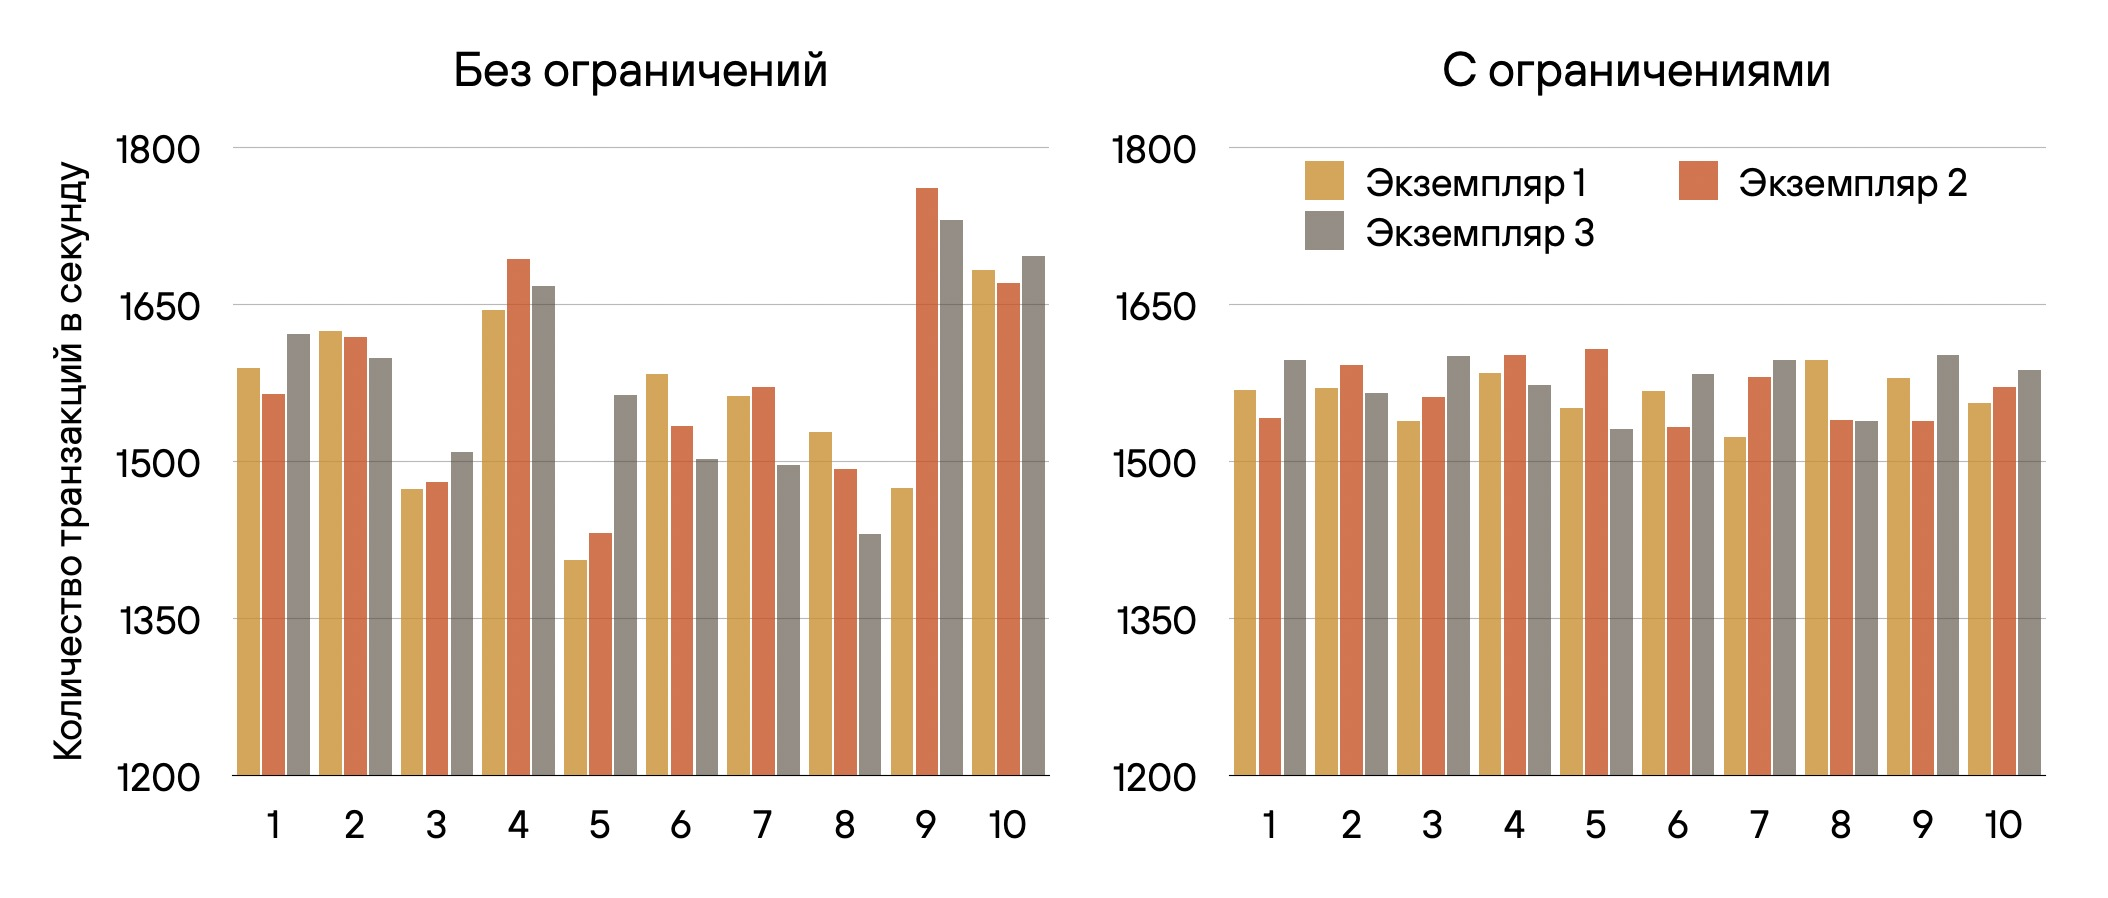
\includegraphics[width=\textwidth]{assets/plot.jpeg}
    \caption{Гистограмма с результатами бенчмарка}
    \label{img:plot}
\end{figure}

На основании полученных результатов, для двух групп тестов были посчитаны выборочное среднее $\hat{\mu}$, размах выборки $R$ и выборочная дисперсия $\hat{\sigma}^2$. Значения округлены до целых. Результаты подсчетов приведены в таблице~\ref{tab:vlasou}.

\begin{table}[H]
\caption{Размах, выборочное среднее и выборочная дисперсия}
\label{tab:vlasou}
\begin{center}
\begin{tabular}{|l|r|r|}
\hline
                 & \multicolumn{1}{c|}{\textbf{Без ограничений}} & \multicolumn{1}{c|}{\textbf{С ограничениями}} \\ \hline
$\hat{\mu}$      & 1573                                          & 1569                                          \\ \hline
$R$              & 356                                           & 84                                            \\ \hline
$\hat{\sigma}^2$ & 8816                                          & 631                                           \\ \hline
\end{tabular}
\end{center}
\end{table}

В тестовом случае с ограниченным дисковым вводом-выводом выборочная дисперсия и размах выборки меньше, чем в случае без ограничений. На основании этого можно сделать вывод о том, что ограничения дискового ввода-вывода могут обеспечить более стабильную производительность СУБД.
